\chapter{Related Work}
\label{ch:related_work}


\section{Tutorial Design}
\label{sec:tutorial_design}

\subsection{DocWizards}
\label{sec:docwizards}
The authors of \emph{DocWizards: A System for Authoring Follow-me Documentation Wizards}~\cite{bergman:docwizards} identify that there are some problems with teaching people to use software (\emph{computer-based procedures}) through documentation alone. Users must find \gls{ui} elements based on documentation descriptions on their own, understand and handle conditional branches, and at the same time keep track of where they are in the process.

\noindent
In their work, they propose the use of a tutorial-like documentation process called \emph{follow-me documentation wizards}, an approach that combines the advantages of conventional wizards and documentation. With their approach, processes are automatically captured from demonstrations made by expert users, and made available to new users in the form of highlighting both text from the documentation (see Fig.~\ref{fig:docwizards}) as well as UI elements for each step.

\begin{figure}[htp]
	\centering
	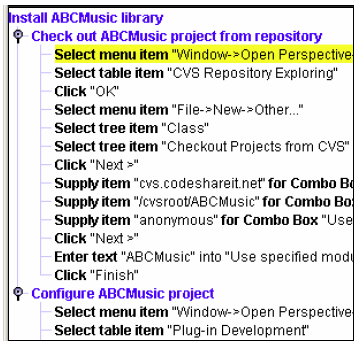
\includegraphics[scale=0.70]{docwizards}
	\caption[\emph{DocWizards} example]{An example of stepwise instructions in \emph{DocWizards}. The current step is highlighted in yellow. \emph{Image source:~\cite{bergman:docwizards}}}
	\label{fig:docwizards}
\end{figure}

\noindent
Finally, a user study is conducted by the authors to evaluate their system, yielding positive results. The usefulness of the \emph{DocWizards} approach has also been verified in a separate study~\cite{gweon:evaluating_docwizards}.

\subsection{Graphstract}
\label{sec:graphstract}
The authors of \emph{Graphstract: Minimal Graphical Help for Computers}~\cite{huang:graphstract} identify problems with the commonly used approach of providing only a textual explanations in software tutorials and help. Users are unlikely to read these explanations carefully enough, if at all. Simply adding screenshots of the \gls{ui} is not an adequate solution, since these usually add far more information than necessary, and thus increase the perceived size and complexity of the explanation. Problems with animation and video are also identified, such as making it difficult for the user to move at their own pace.

\noindent
Instead of relying on text-only descriptions or simple screenshots, the authors propose the use of graphical help in the form of partial screenshots, combined to show a complete sequence of actions required to perform a task (see Fig.~\ref{fig:graphstract}). This approach provides graphical help directly mapped to the \gls{ui}, without adding a lot of extra information. Additionally, the whole sequence is presented in a small space, making it easy to get an overview.

\begin{figure}[htp]
	\centering
	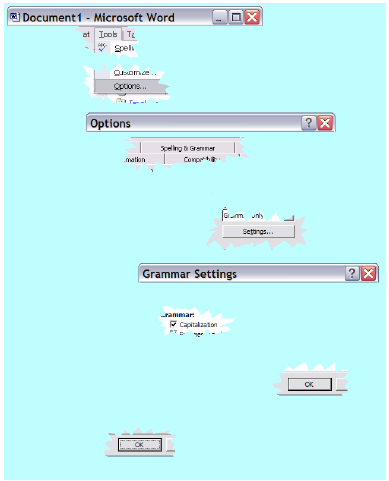
\includegraphics[scale=0.70]{graphstract}
	\caption[\emph{Graphstract} example]{An example of stepwise instructions in \emph{Graphstract} in the form of screenshot snippets, showing the steps required to toggle auto-capitalization in Microsoft Word. \emph{Image source:~\cite{huang:graphstract}}}
	\label{fig:graphstract}
\end{figure}

\noindent
Three iterations of user studies on a prototype is conducted by the authors, showing that \emph{Graphstract} performs better than conventional approaches overall, if not in all cases. They also conclude that adding text to the images is useful in many situations, despite their approach relying on graphical help only.

\subsection{Toolclips}
\label{sec:toolclips}
The authors of \emph{ToolClips: An Investigation of Contextual
Video Assistance for Functionality Understanding}~\cite{grossman:toolclips} explore the \emph{learnability} of software products, more specifically relating to the concept of \emph{understanding} how to properly use functionality (see~\cite{grossman:software_learnability}). They identify problems with existing approaches based on both text and videos, where information is provided outside the context of the \gls{ui} in question. The authors also assess that regular tooltips, which provide the user with a short in-context description of what a \gls{ui} element does, do not provide a sufficient level of detail for complex tools.

\noindent


\begin{figure}[htp]
	\centering
	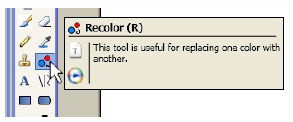
\includegraphics[scale=0.80]{toolclips}
	\caption[\emph{ToolClips} example]{An example of a \emph{ToolClip}, appearing as a regular tooltip, but with additional functionality for media. \emph{Image source:~\cite{grossman:toolclips}}}
	\label{fig:toolclips}
\end{figure}


\subsection{Photo Tutorials}




\section{Game-based Learning}
\label{sec:rel_game_based_learning}

\subsection{CodeSpells}
Learn Java programming

\subsection{Karel the Robot}
Learn Java programming

\subsection{Kahoot}
Not relevant?

